\chapter{NTP (Network Time Protocol)}\label{ntp-network-time-protocol}

WHY IS TIME IMPORTANT FOR NETWORK DEVICES?

\begin{itemize}
\tightlist
\item
  All DEVICES have an INTERNAL CLOCK (ROUTERS, SWITCHES, PCs, etc)
\item
  In CISCO IOS, you can view the time with the
  \passthrough{\lstinline!show clock!} command
\end{itemize}

\begin{figure}
\centering
\pandocbounded{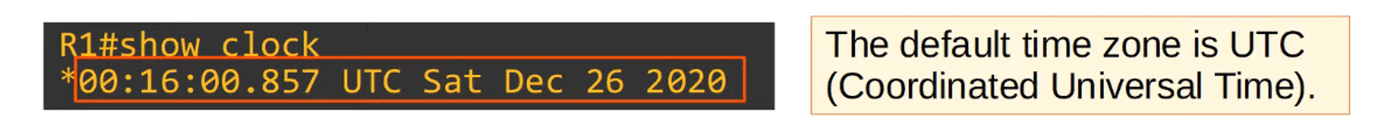
\includegraphics[keepaspectratio,alt={image}]{images/38-ntp/img-001.png}}
\end{figure}

\begin{itemize}
\tightlist
\item
  If you use the \passthrough{\lstinline!show clock detail!} command,
  you can see the TIME SOURCE
\end{itemize}

\begin{figure}
\centering
\pandocbounded{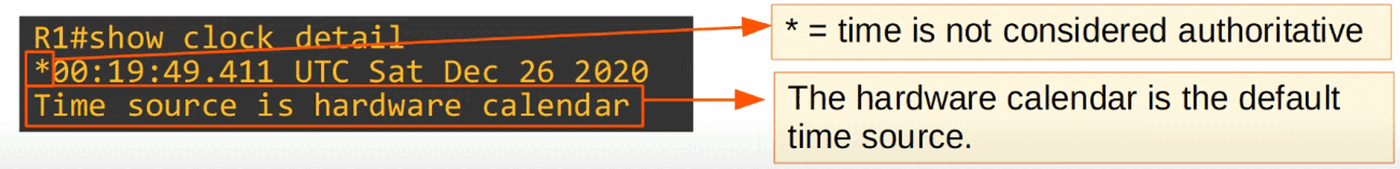
\includegraphics[keepaspectratio,alt={image}]{images/38-ntp/img-002.png}}
\end{figure}

\begin{itemize}
\item
  The INTERNAL HARDWARE CLOCK of a DEVICE will ``drift' over time, so
  it's NOT the ideal time source.
\item
  From a CCNA perspective, the most important reason to have accurate
  time on a DEVICE is to have ACCURATE logs for troubleshooting
\item
  \textbf{Syslog}, the protocol used to keep device logs, will be
  covered in a later video
\end{itemize}

Command: \passthrough{\lstinline!show logging!}

\begin{figure}
\centering
\pandocbounded{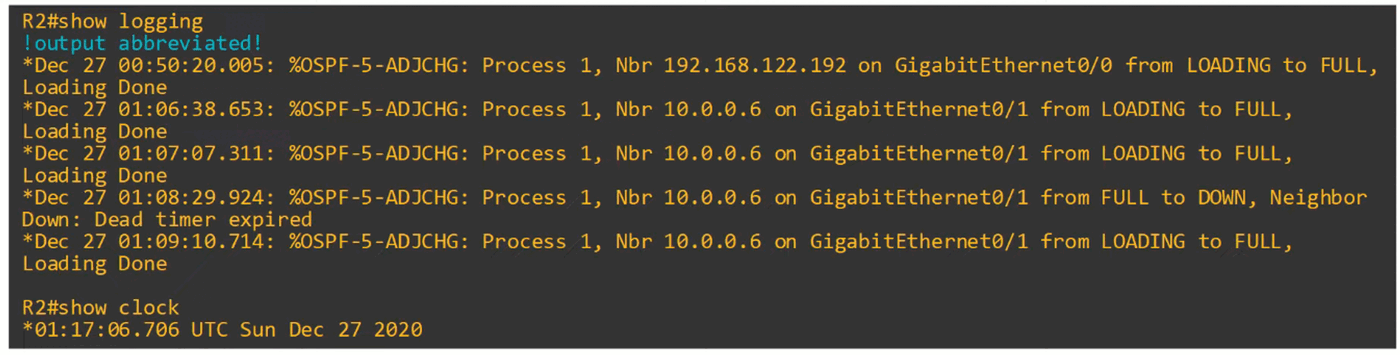
\includegraphics[keepaspectratio,alt={image}]{images/38-ntp/img-003.png}}
\end{figure}

Note : R3's time stamp is completely different than R2's !!!

\begin{figure}
\centering
\pandocbounded{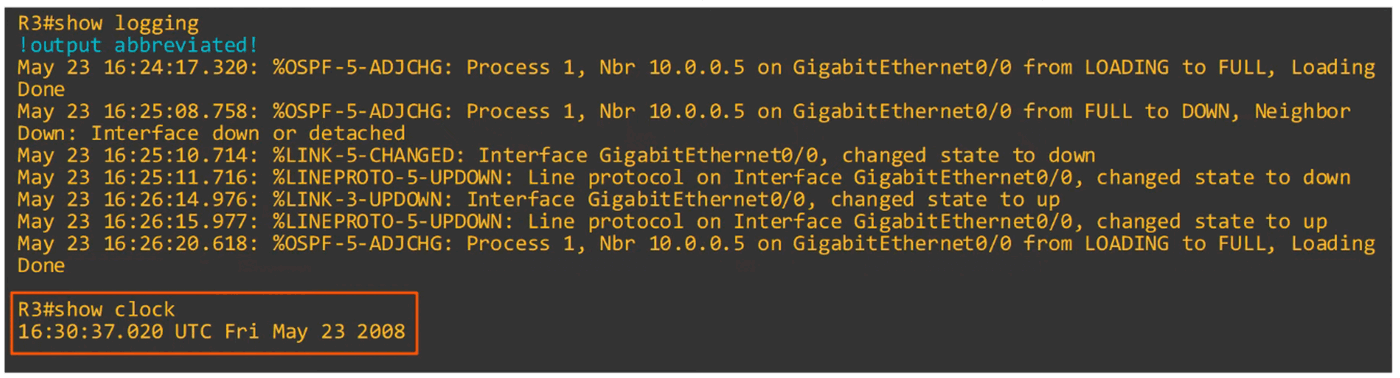
\includegraphics[keepaspectratio,alt={image}]{images/38-ntp/img-004.png}}
\end{figure}

\section{Manual Time Configuration}\label{manual-time-configuration}

\begin{itemize}
\tightlist
\item
  You can manually configure the TIME on the DEVICE with the
  \passthrough{\lstinline!clock set!} command
\end{itemize}

\begin{figure}
\centering
\pandocbounded{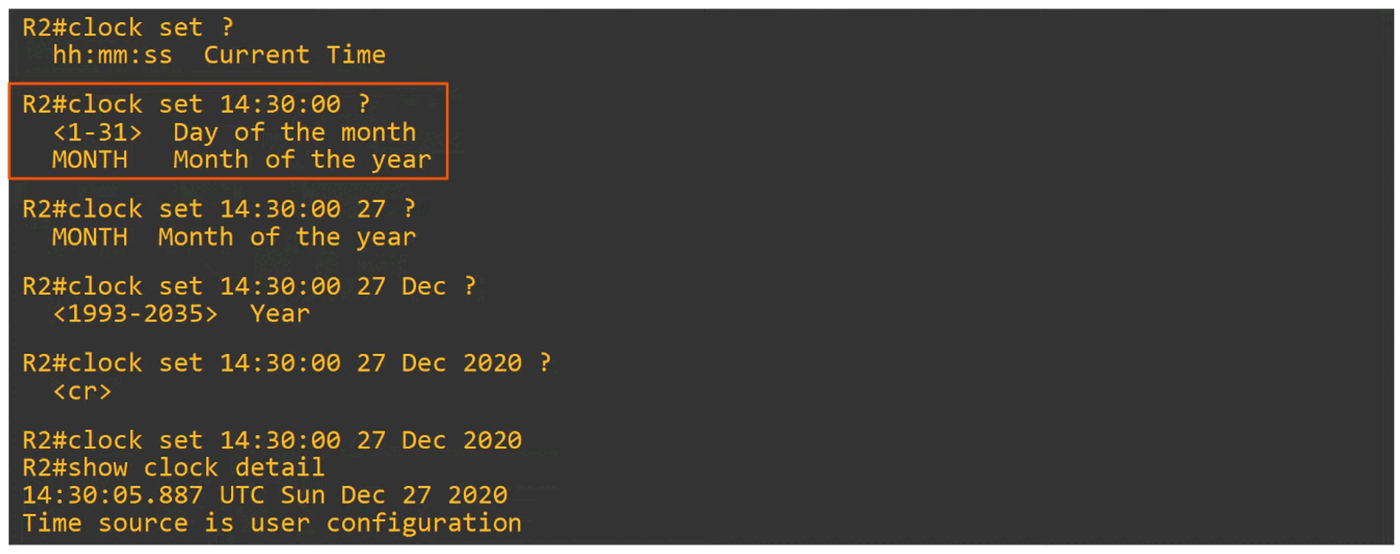
\includegraphics[keepaspectratio,alt={image}]{images/38-ntp/img-005.png}}
\end{figure}

\begin{itemize}
\tightlist
\item
  Although the HARDWARE CALENDAR (built-in clock) is the DEFAULT
  time-source, the HARDWARE CLOCK and SOFTWARE CLOCK are separate and
  can be configured separately.
\end{itemize}

\section{Hardware Clock (Calendar)
Configuration}\label{hardware-clock-calendar-configuration}

\begin{itemize}
\tightlist
\item
  You can MANUALLY configure the HARDWARE CLOCK with the
  \passthrough{\lstinline!calendar set!} command
\end{itemize}

\begin{figure}
\centering
\pandocbounded{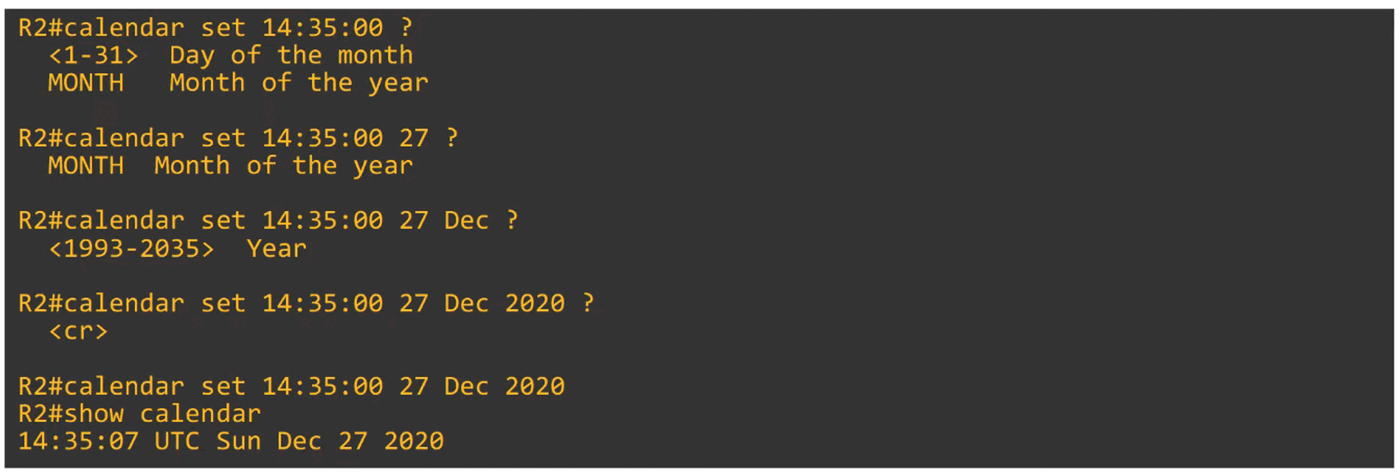
\includegraphics[keepaspectratio,alt={image}]{images/38-ntp/img-006.png}}
\end{figure}

\begin{itemize}
\tightlist
\item
  Typically, you will want to SYNCHRONIZE the `clock' and `calendar'
\item
  Use the command \passthrough{\lstinline!clock update-calendar!} to
  sync the calendar to the clock's time
\item
  Use the command \passthrough{\lstinline!clock read-calendar!} to sync
  the clock to the calendar's time
\end{itemize}

\begin{figure}
\centering
\pandocbounded{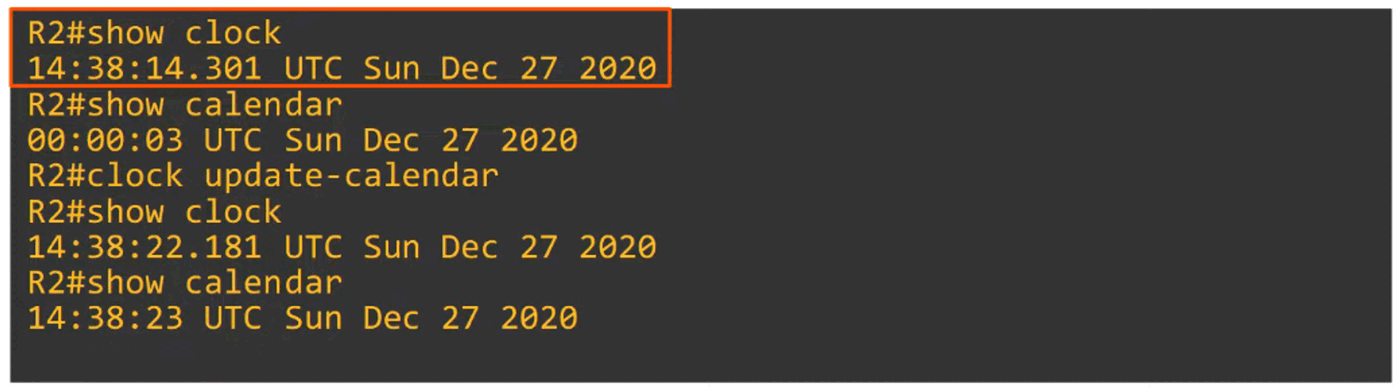
\includegraphics[keepaspectratio,alt={image}]{images/38-ntp/img-007.png}}
\end{figure}

\begin{figure}
\centering
\pandocbounded{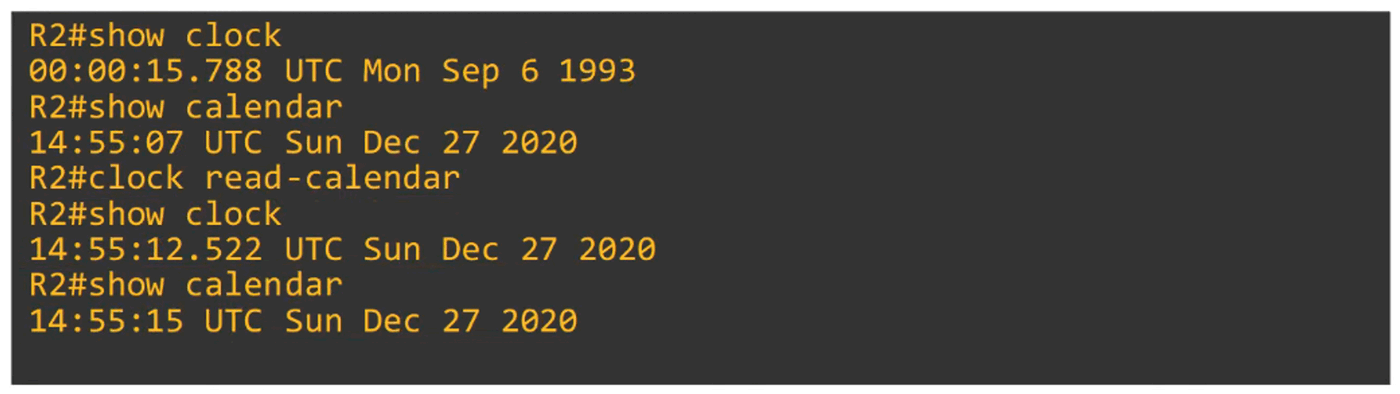
\includegraphics[keepaspectratio,alt={image}]{images/38-ntp/img-008.png}}
\end{figure}

\section{Configuring the Time Zone}\label{configuring-the-time-zone}

\begin{itemize}
\tightlist
\item
  You can configure the time zone with the
  \passthrough{\lstinline!clock timezone!} command
\end{itemize}

\begin{figure}
\centering
\pandocbounded{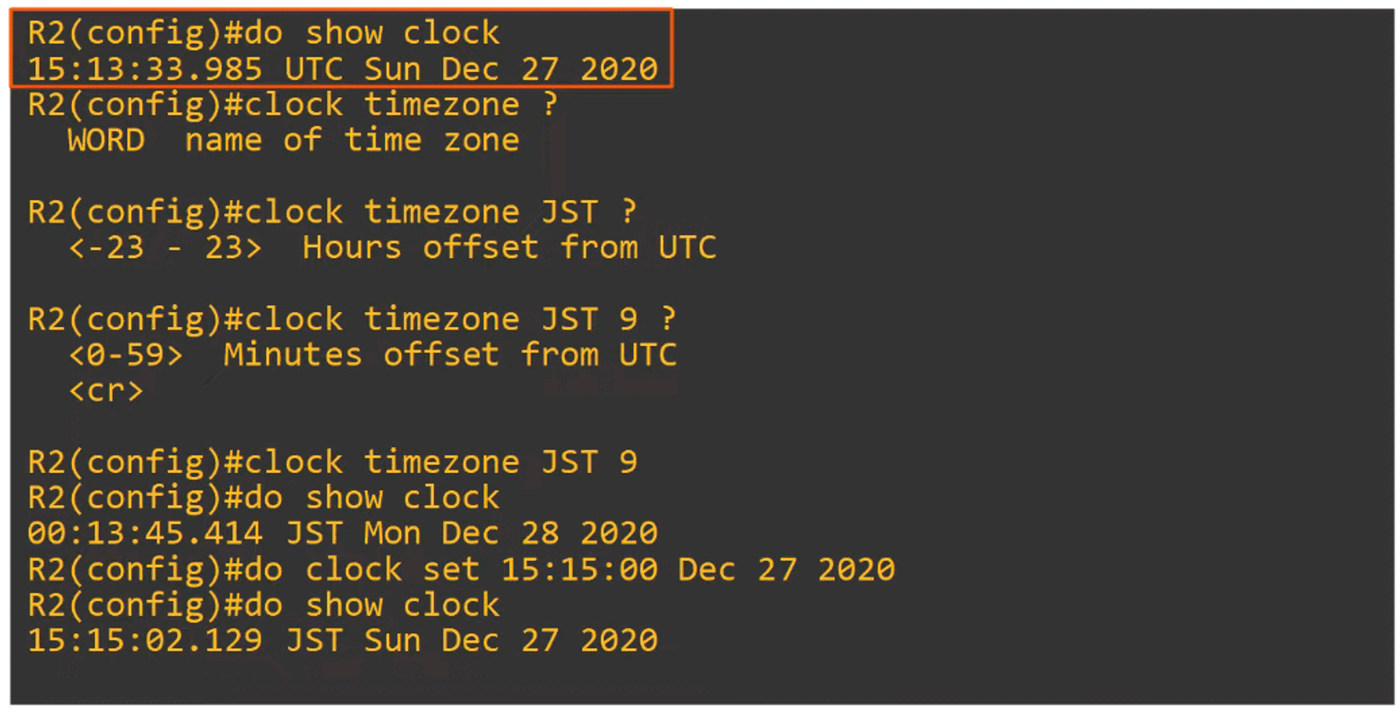
\includegraphics[keepaspectratio,alt={image}]{images/38-ntp/img-009.png}}
\end{figure}

\section{Daylight Saving Time (Summer
Time)}\label{daylight-saving-time-summer-time}

\begin{figure}
\centering
\pandocbounded{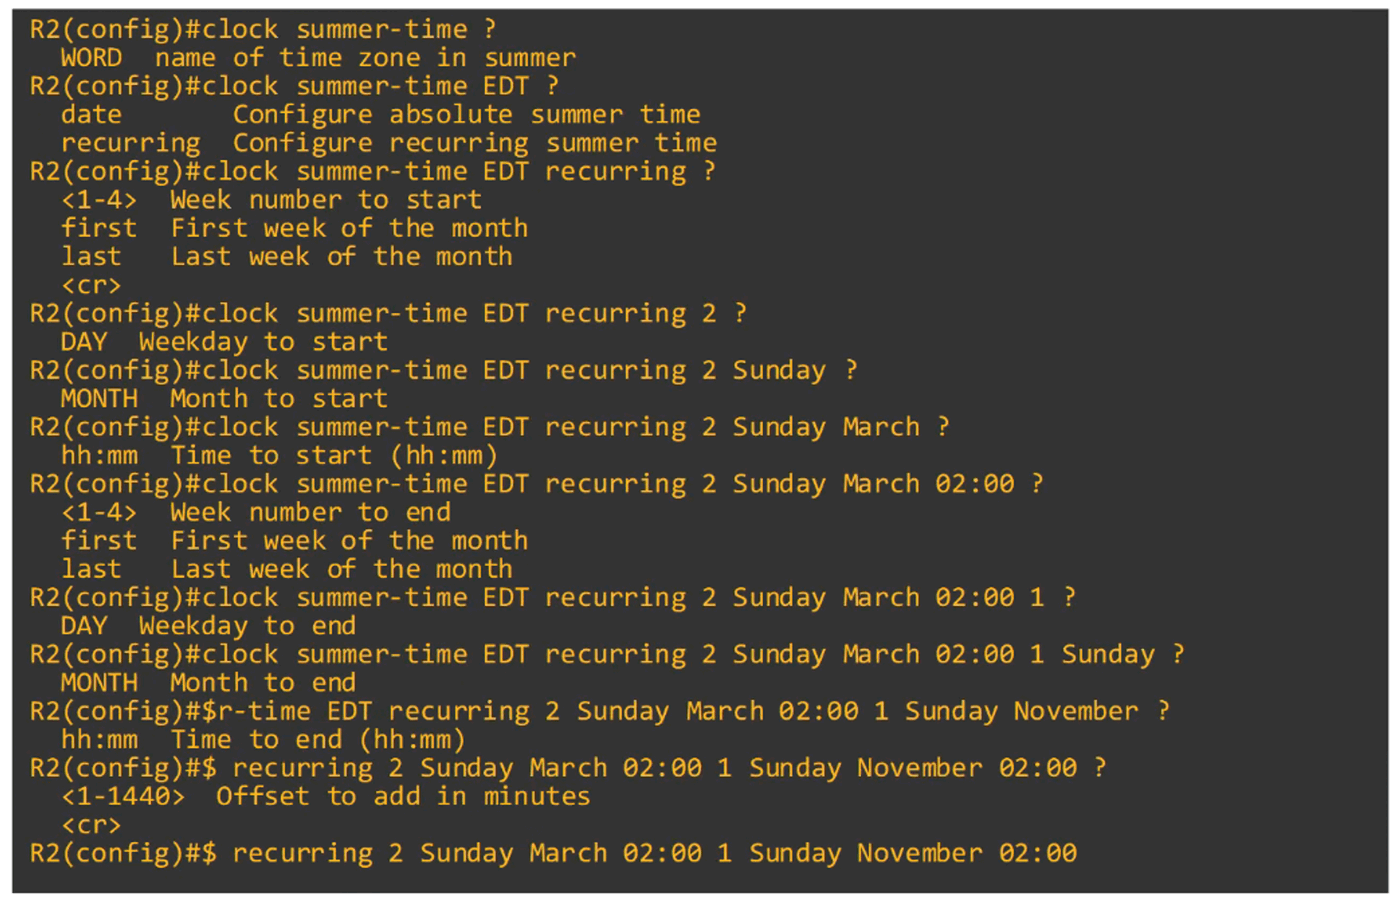
\includegraphics[keepaspectratio,alt={image}]{images/38-ntp/img-010.png}}
\end{figure}

\begin{figure}
\centering
\pandocbounded{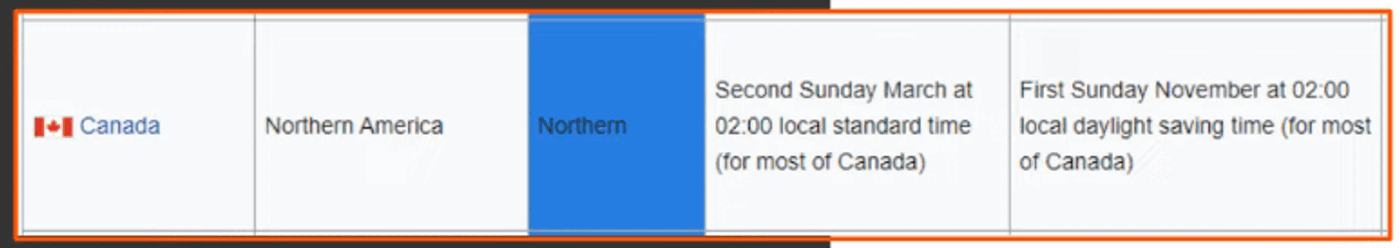
\includegraphics[keepaspectratio,alt={image}]{images/38-ntp/img-011.png}}
\end{figure}

Full command :

\passthrough{\lstinline!R1(config)\# clock summer-time EDT recurring 2 Sunday March 02:00 1 Sunday November 02:00!}

This covers the START of Daylight Savings and the end of Daylight
Savings

\section{Summary of Commands}\label{summary-of-commands}

\begin{figure}
\centering
\pandocbounded{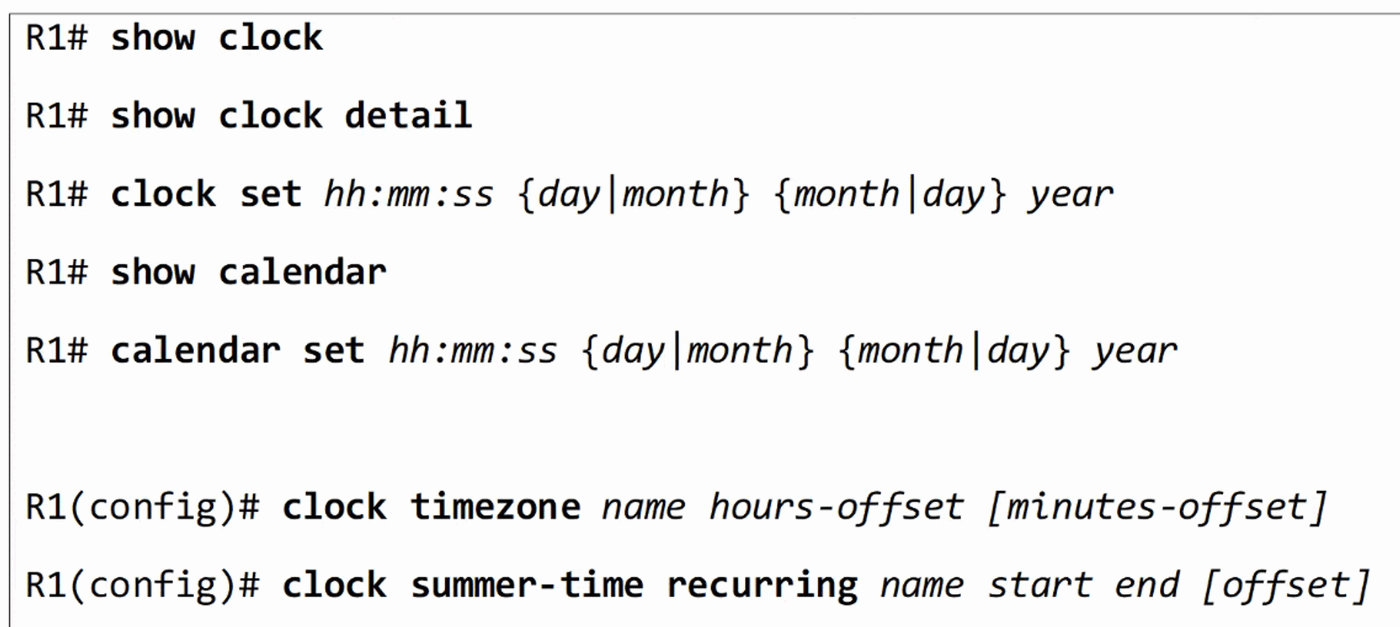
\includegraphics[keepaspectratio,alt={image}]{images/38-ntp/img-012.png}}
\end{figure}

\section{NTP Basics}\label{ntp-basics}

\begin{itemize}
\tightlist
\item
  Manually configuring the time on DEVICES is NOT Scalable
\item
  The manually configured clocks will ``drift'', resulting in inaccurate
  time
\item
  NTP (Network Time Protocol) allows AUTOMATIC synchronization of TIME
  over a NETWORK
\item
  NTP CLIENTS request the TIME from NTP SERVERS
\item
  A DEVICE can be an NTP SERVER and an NTP CLIENT at the same time
\item
  NTP allows accuracy of TIME with \textasciitilde1 millisecond if the
  NTP SERVER is in the same LAN - OR within \textasciitilde50
  milliseconds if connecting to the NTP SERVER over a WAN / the INTERNET
\item
  Some NTP SERVERS are `better' than others. The `distance' of an NTP
  SERVER from the original \textbf{reference clock} is called
  \textbf{stratum}
\end{itemize}

\begin{tipbox}

NTP uses UDP port 123 to communicate

\end{tipbox}

\section{Reference Clock}\label{reference-clock}

\begin{itemize}
\tightlist
\item
  A REFERENCE CLOCK is usually a VERY accurate time device like an
  ATOMIC CLOCK or GPS CLOCK
\item
  REFERENCE CLOCKS are \textbf{stratum 0} within the NTP hierarchy
\item
  NTP SERVERS directly connected to REFERENCE CLOCKS are \textbf{stratum
  1}
\end{itemize}

\begin{figure}
\centering
\pandocbounded{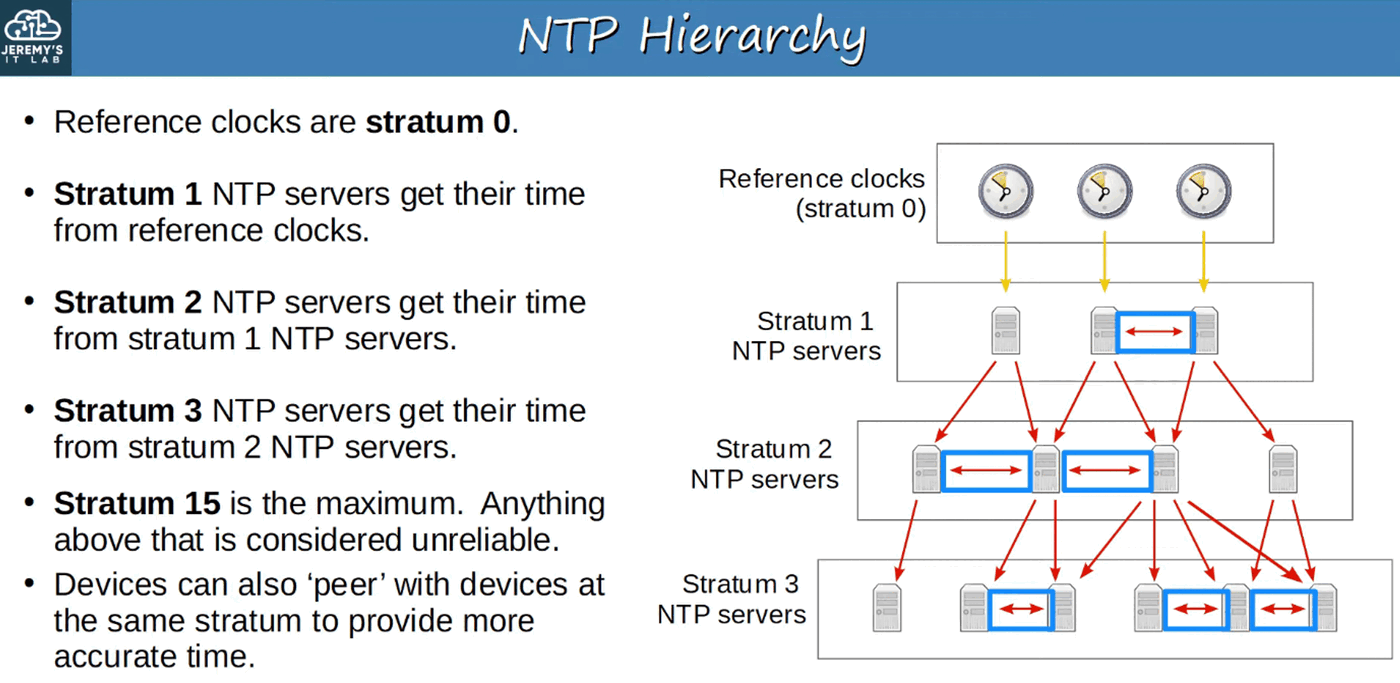
\includegraphics[keepaspectratio,alt={image}]{images/38-ntp/img-013.png}}
\end{figure}

(Peering with Devices is called \ldots)

\begin{figure}
\centering
\pandocbounded{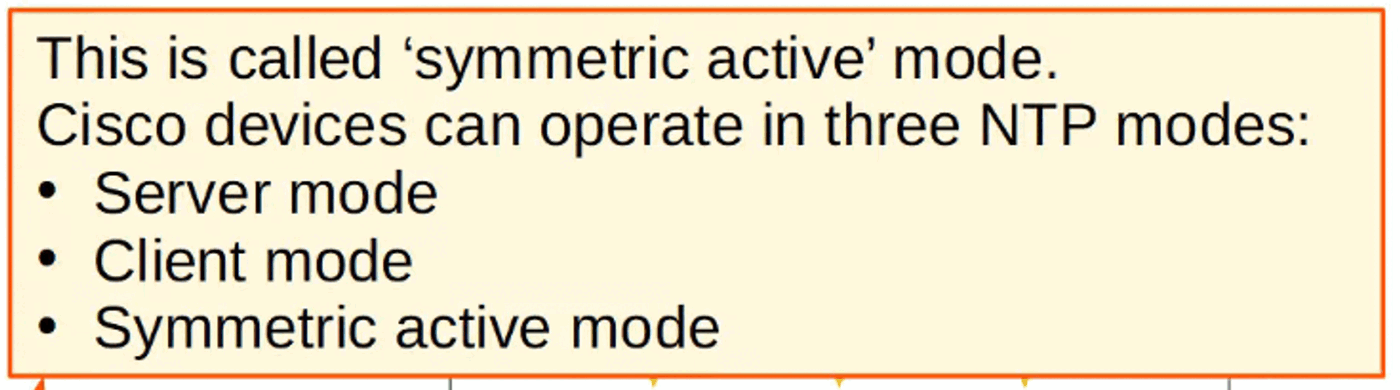
\includegraphics[keepaspectratio,alt={image}]{images/38-ntp/img-014.png}}
\end{figure}

\begin{itemize}
\tightlist
\item
  An NTP CLIENT can SYNC to MULTIPLE NTP SERVERS
\end{itemize}

\begin{figure}
\centering
\pandocbounded{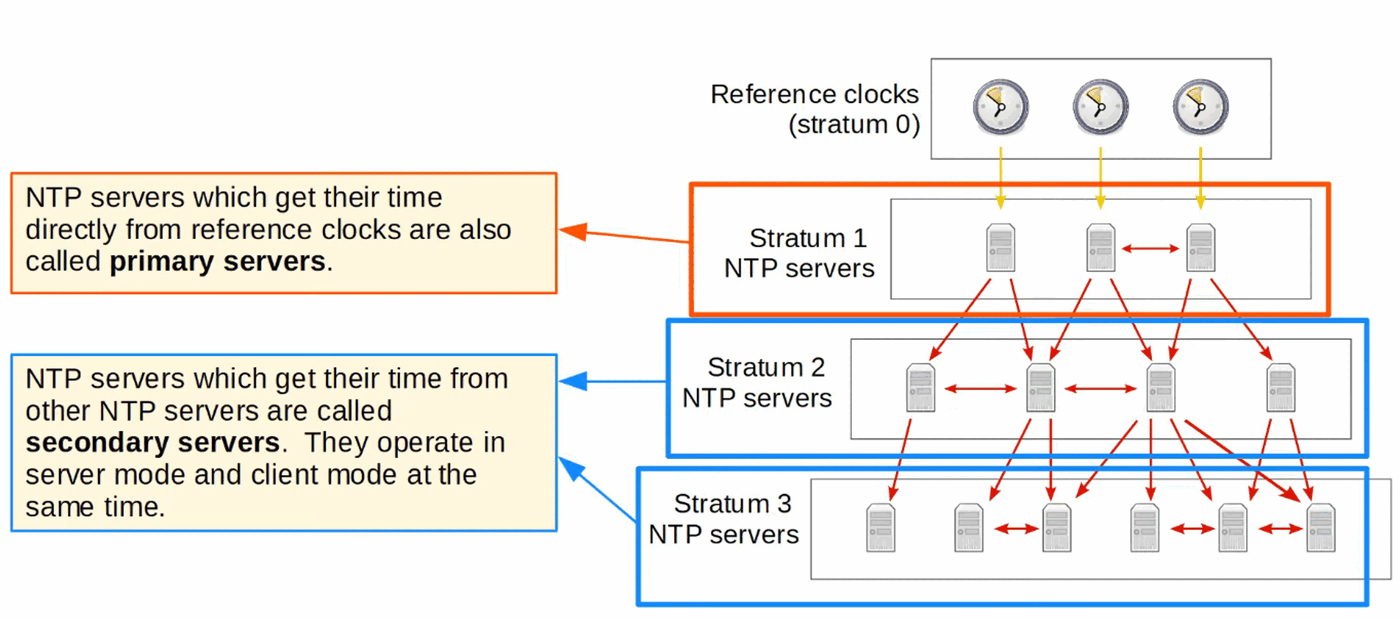
\includegraphics[keepaspectratio,alt={image}]{images/38-ntp/img-015.png}}
\end{figure}

\section{NTP Configuration}\label{ntp-configuration}

\begin{figure}
\centering
\pandocbounded{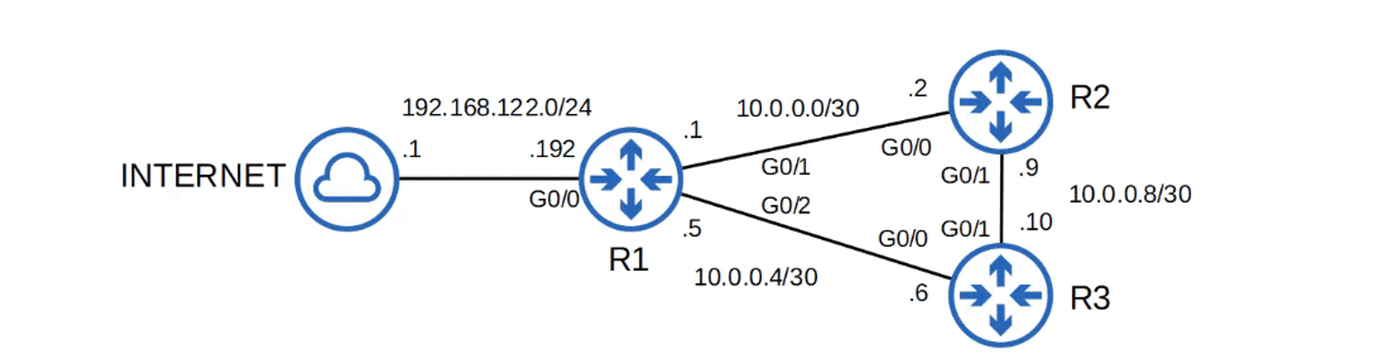
\includegraphics[keepaspectratio,alt={image}]{images/38-ntp/img-016.png}}
\end{figure}

\begin{figure}
\centering
\pandocbounded{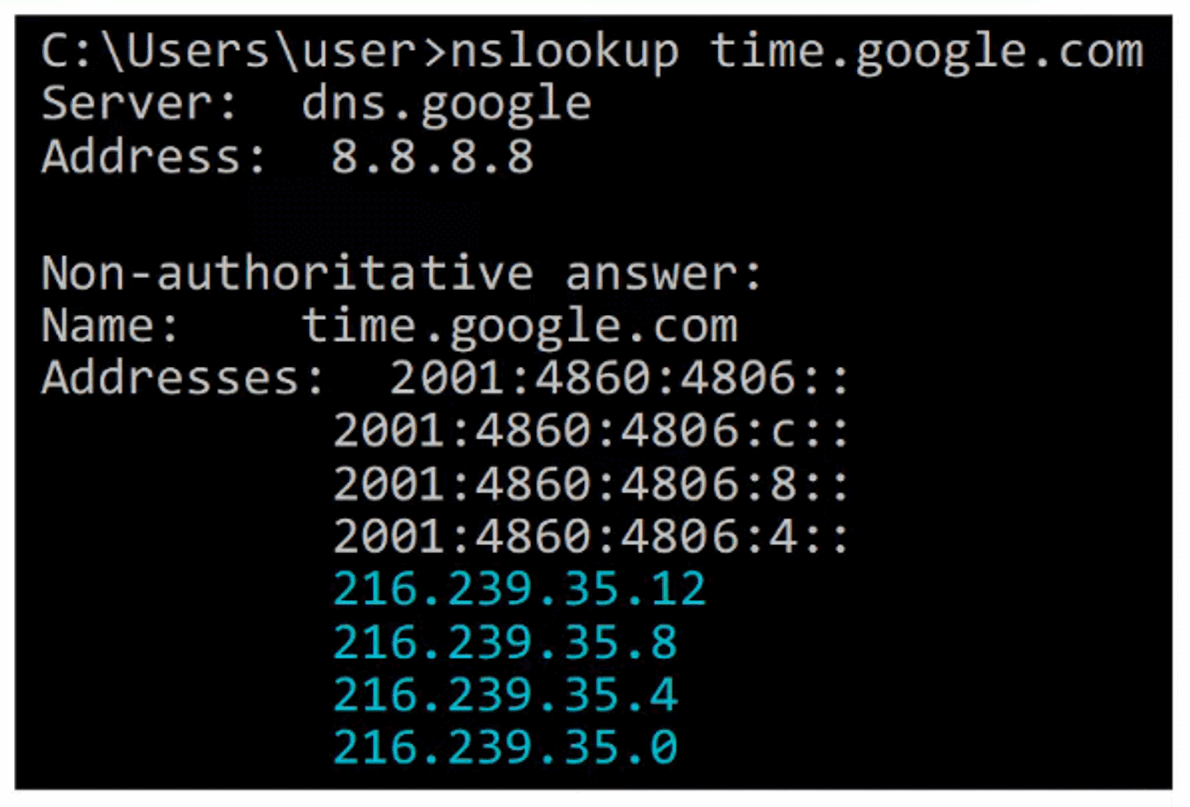
\includegraphics[keepaspectratio,alt={image}]{images/38-ntp/img-017.png}}
\end{figure}

\begin{figure}
\centering
\pandocbounded{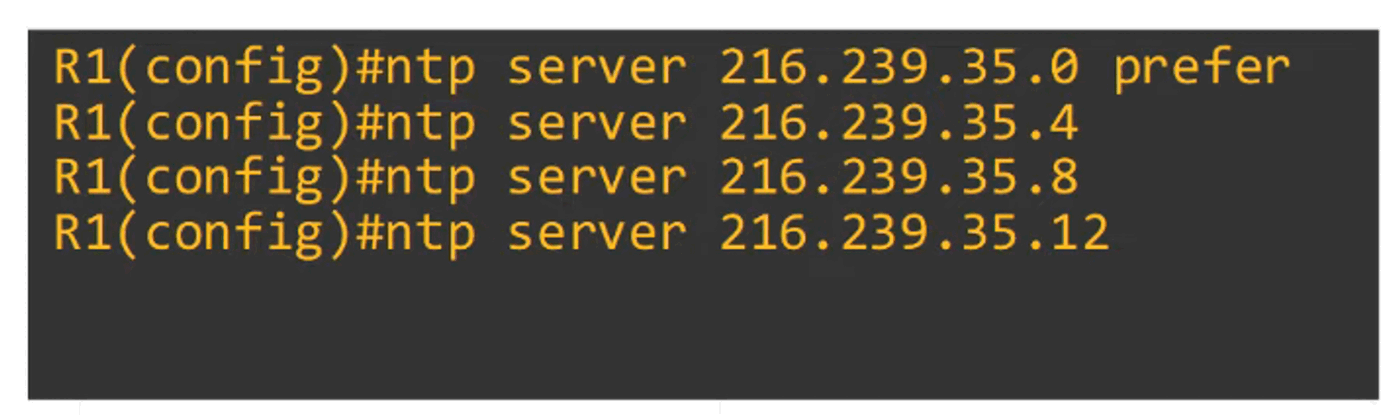
\includegraphics[keepaspectratio,alt={image}]{images/38-ntp/img-018.png}}
\end{figure}

Using key argument ``prefer'' makes a given server the PREFERRED SERVER

(To show configuration servers)

\begin{figure}
\centering
\pandocbounded{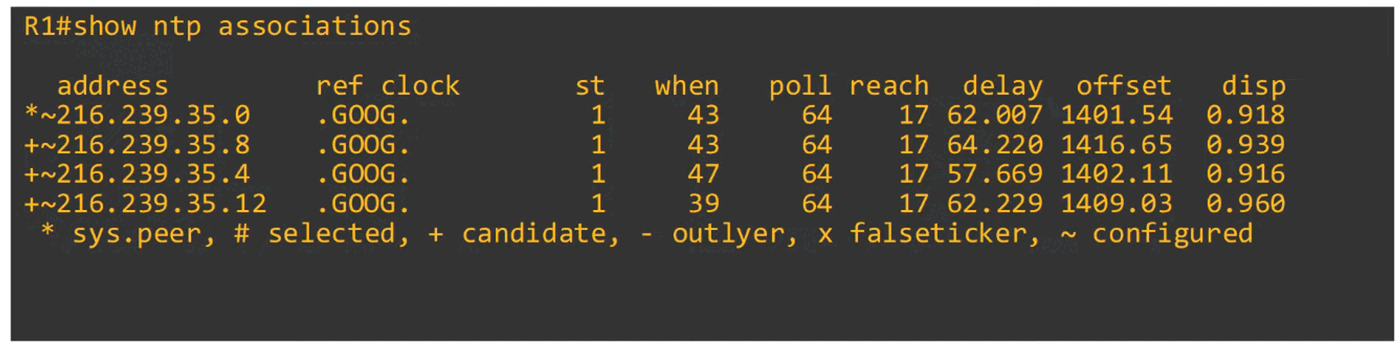
\includegraphics[keepaspectratio,alt={image}]{images/38-ntp/img-019.png}}
\end{figure}

\passthrough{\lstinline!sys.peer!} = This is the SERVER that the current
ROUTER (R1) is being synchronized to

\passthrough{\lstinline!st!} = Stratum Tier

(To show NTP Status)

\begin{figure}
\centering
\pandocbounded{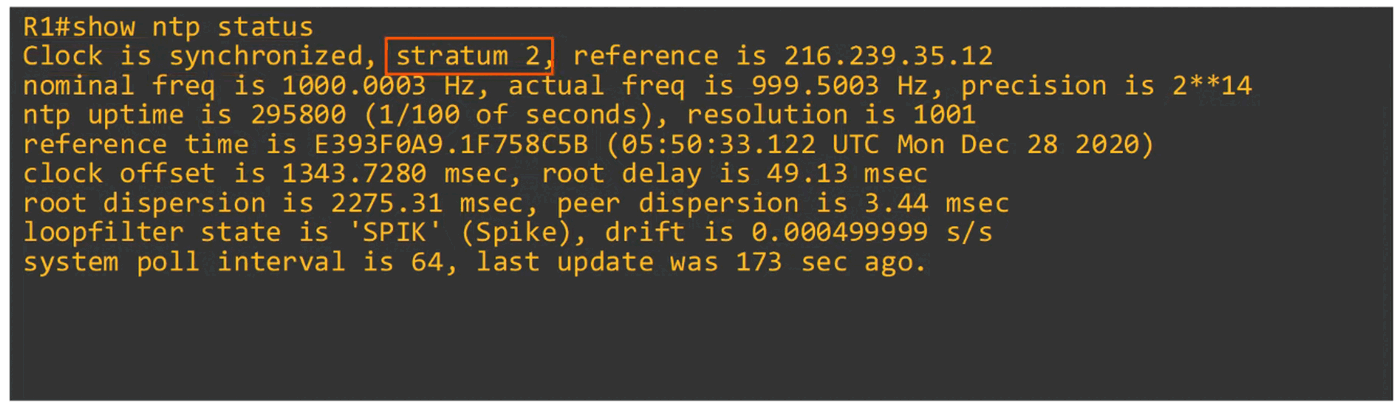
\includegraphics[keepaspectratio,alt={image}]{images/38-ntp/img-020.png}}
\end{figure}

\passthrough{\lstinline!stratum 2!} because it's synchronizing from
Google (stratum 1)

(To show NTP clock details)

\begin{figure}
\centering
\pandocbounded{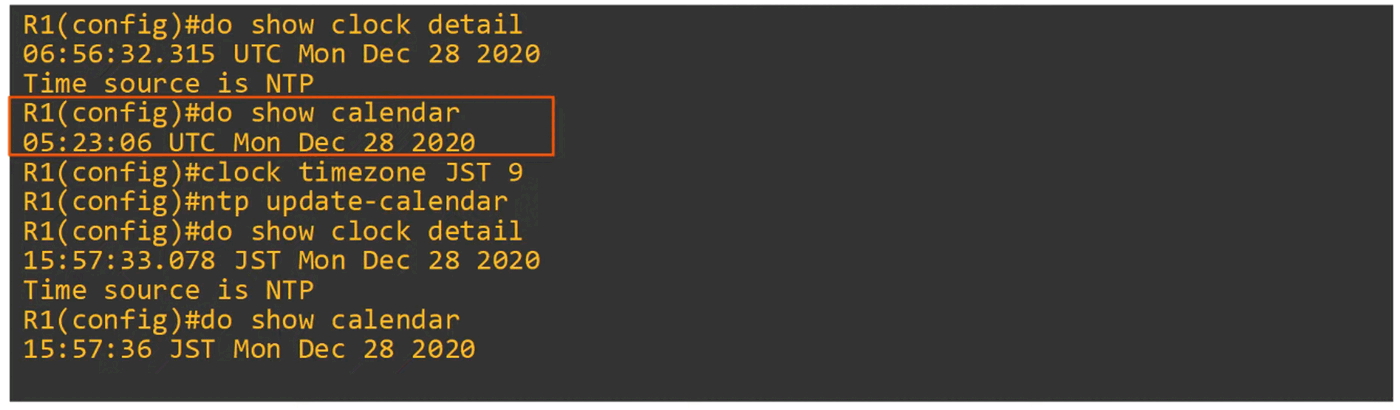
\includegraphics[keepaspectratio,alt={image}]{images/38-ntp/img-021.png}}
\end{figure}

This command configures the ROUTER to update the HARDWARE CLOCK
(Calendar) with the time learned via NTP

\passthrough{\lstinline!R1(config)\# ntp update-calendar!}

The HARDWARE CLOCK tracks the DATE and TIME on the DEVICE - even if it
restarts, power is lost, etc.

When the SYSTEM is restarted, the HARDWARE CLOCK is used to INITIALIZE
the SOFTWARE CLOCK

\section{Configure a Loopback Interface for an NTP
Server}\label{configure-a-loopback-interface-for-an-ntp-server}

\begin{figure}
\centering
\pandocbounded{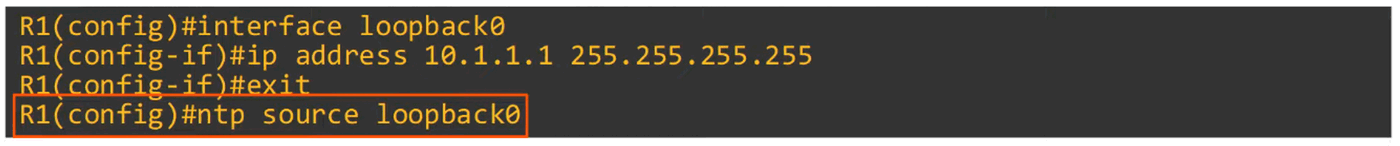
\includegraphics[keepaspectratio,alt={image}]{images/38-ntp/img-022.png}}
\end{figure}

Why configure a LOOPBACK DEVICE on R1 for NTP ?

If one of R1's ROUTER INTERFACES goes down, it will still be accessible
via R3's ROUTING path

\begin{figure}
\centering
\pandocbounded{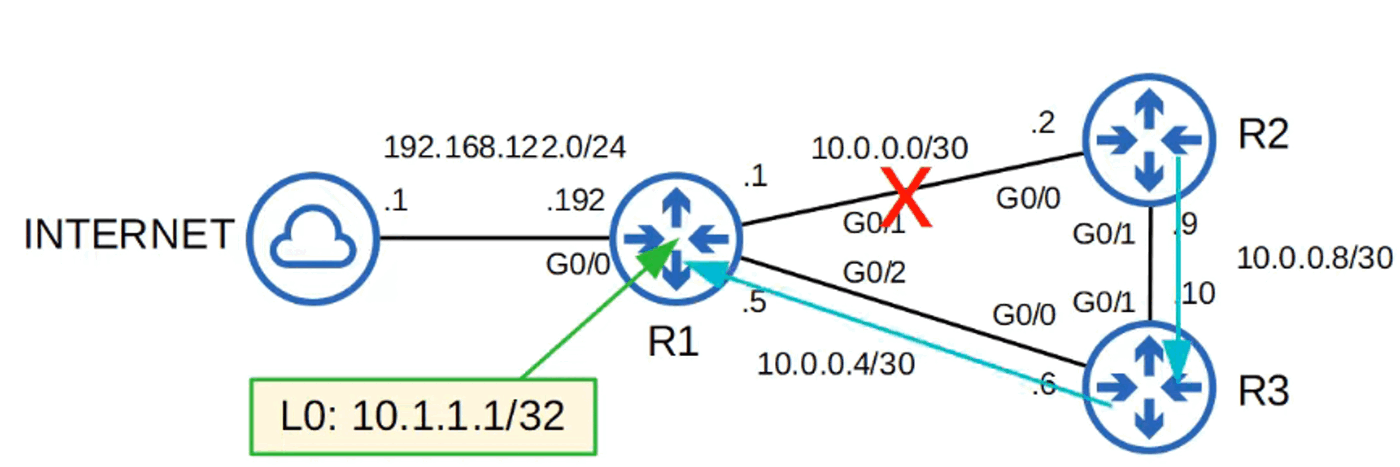
\includegraphics[keepaspectratio,alt={image}]{images/38-ntp/img-023.png}}
\end{figure}

SET NTP SERVER for R2 using the LOOPBACK INTERFACE on R1

\begin{figure}
\centering
\pandocbounded{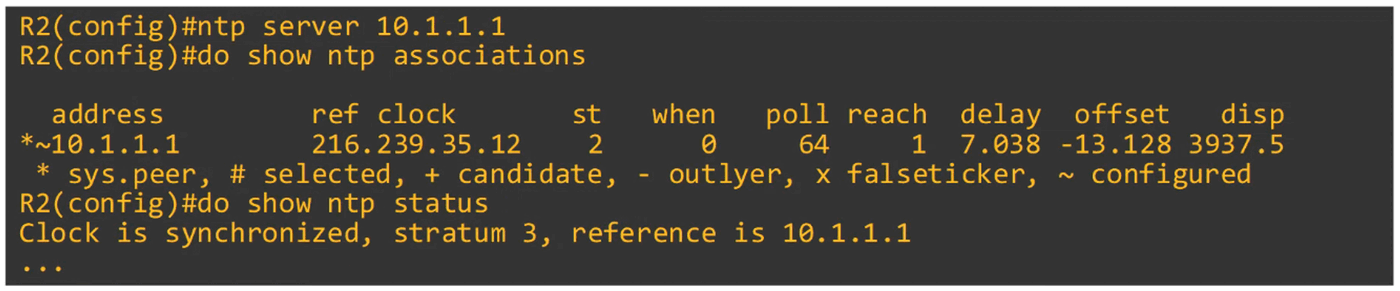
\includegraphics[keepaspectratio,alt={image}]{images/38-ntp/img-024.png}}
\end{figure}

SETTING R3 NTP SOURCE SERVERS using R1 and R2

\begin{figure}
\centering
\pandocbounded{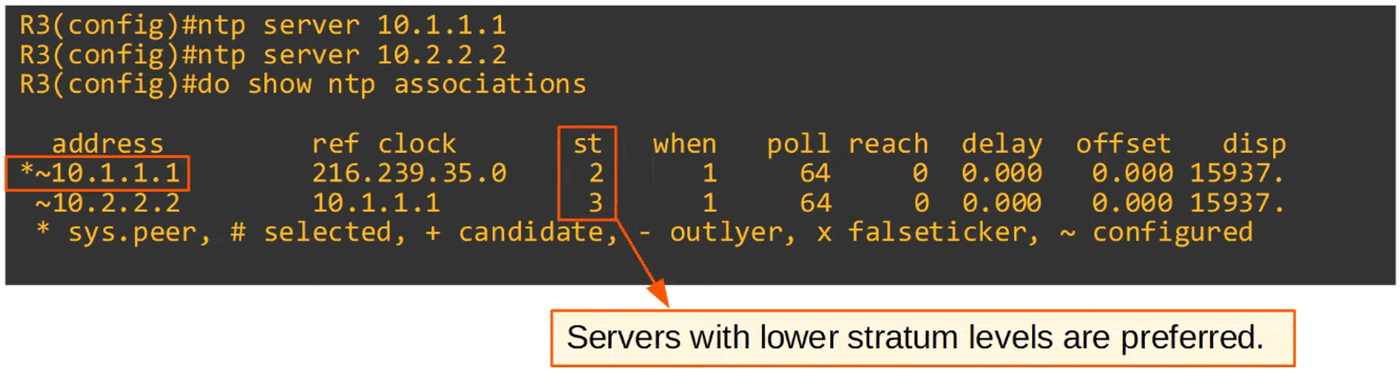
\includegraphics[keepaspectratio,alt={image}]{images/38-ntp/img-025.png}}
\end{figure}

NOTE : R1 has PREFERENCE because it's STRATUM TIER is HIGHER than R2s

\section{Configuring NTP Server Mode}\label{configuring-ntp-server-mode}

\begin{figure}
\centering
\pandocbounded{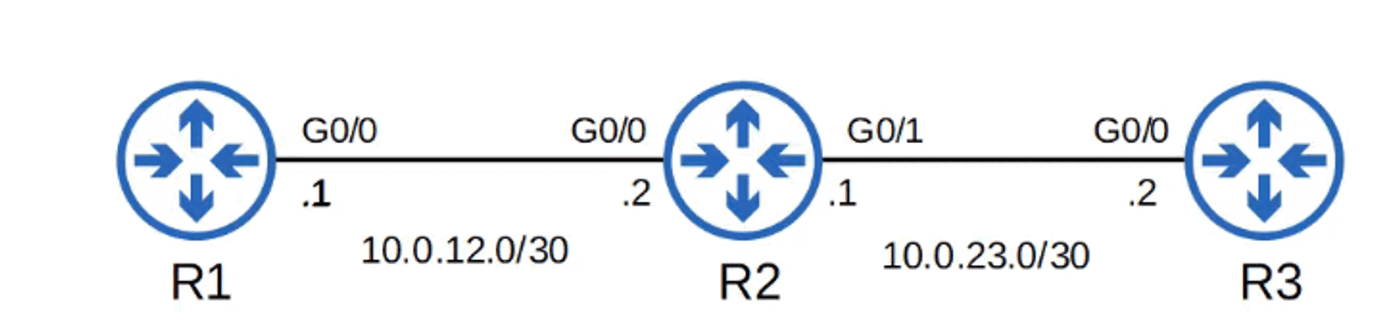
\includegraphics[keepaspectratio,alt={image}]{images/38-ntp/img-026.png}}
\end{figure}

\begin{figure}
\centering
\pandocbounded{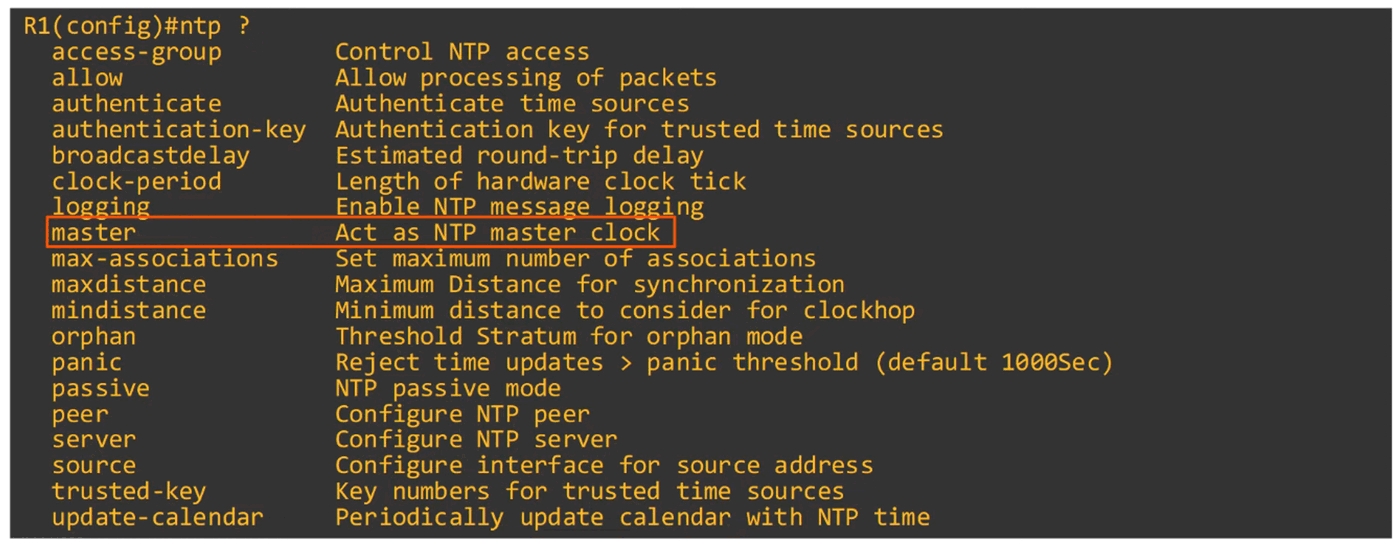
\includegraphics[keepaspectratio,alt={image}]{images/38-ntp/img-027.png}}
\end{figure}

\begin{figure}
\centering
\pandocbounded{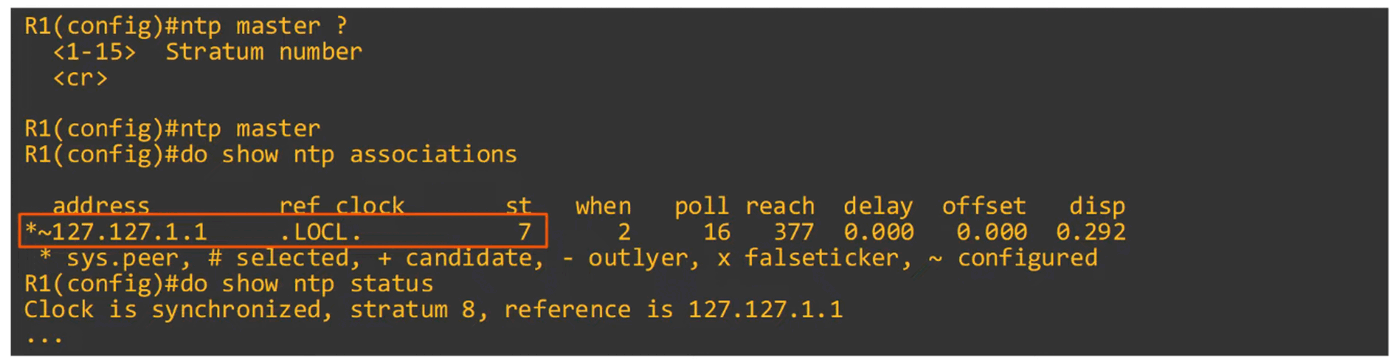
\includegraphics[keepaspectratio,alt={image}]{images/38-ntp/img-028.png}}
\end{figure}

\begin{figure}
\centering
\pandocbounded{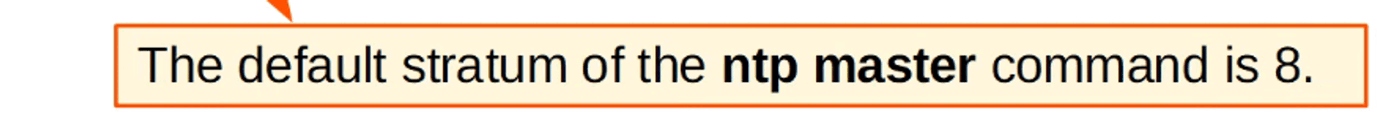
\includegraphics[keepaspectratio,alt={image}]{images/38-ntp/img-029.png}}
\end{figure}

\begin{figure}
\centering
\pandocbounded{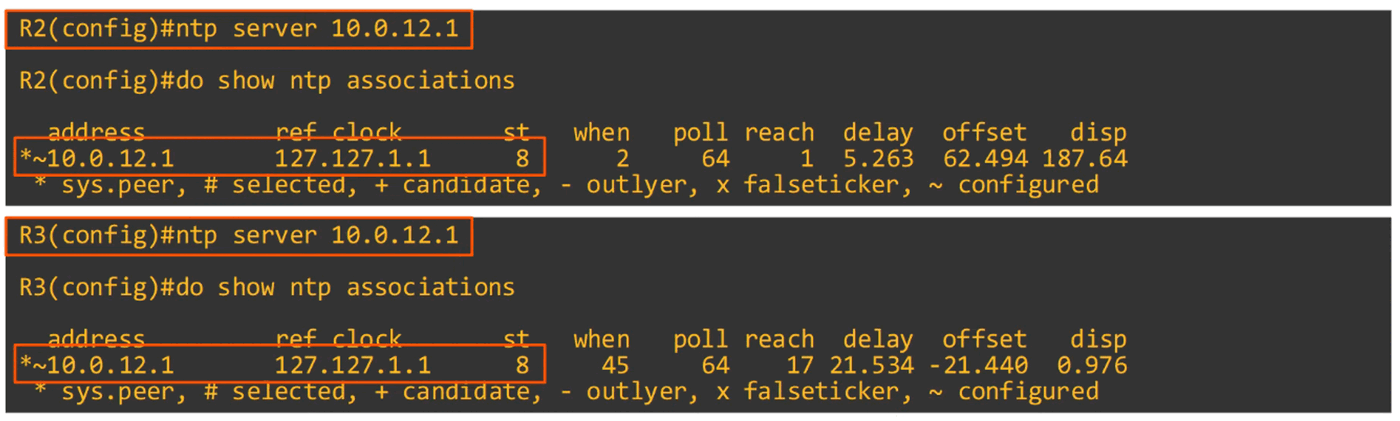
\includegraphics[keepaspectratio,alt={image}]{images/38-ntp/img-030.png}}
\end{figure}

\section{Configuring NTP Symmetric Active
Mode}\label{configuring-ntp-symmetric-active-mode}

Command to configure NTP SYMMETRIC MODE
\passthrough{\lstinline!R2(config)\#ntp peer <peer ip address>!}

\begin{figure}
\centering
\pandocbounded{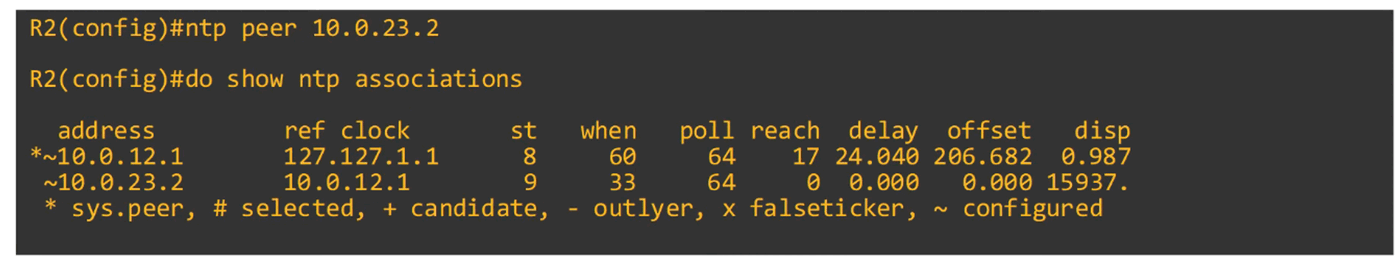
\includegraphics[keepaspectratio,alt={image}]{images/38-ntp/img-031.png}}
\end{figure}

\begin{figure}
\centering
\pandocbounded{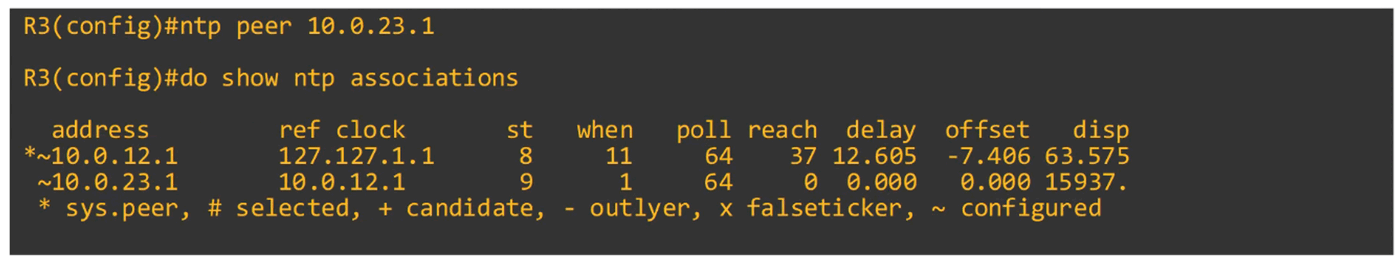
\includegraphics[keepaspectratio,alt={image}]{images/38-ntp/img-032.png}}
\end{figure}

\section{Configure NTP
Authentication}\label{configure-ntp-authentication}

\begin{itemize}
\tightlist
\item
  NTP AUTHENTICATION can be configured, although it is OPTIONAL
\item
  It allows NTP CLIENTS to ensure they only sync to the intended SERVERS
\item
  To CONFIGURE NTP AUTHENTICATION:

  \begin{itemize}
  \tightlist
  \item
    \passthrough{\lstinline!ntp authenticate!} (Enables NTP
    AUTHENTICATION)
  \item
    \passthrough{\lstinline!ntp authenticate-key *key-number* md5 *key*!}
    (Create the NTP AUTHENTICATION Key(s))
  \item
    \passthrough{\lstinline!ntp trusted-key *key-number!}* (Specify the
    Trusted Key(s))
  \item
    \passthrough{\lstinline!ntp server *ip-address* key *key-number!}*
    (Specify which key to use for the server)
  \end{itemize}
\end{itemize}

\section{Example Configurations}\label{example-configurations}

\begin{figure}
\centering
\pandocbounded{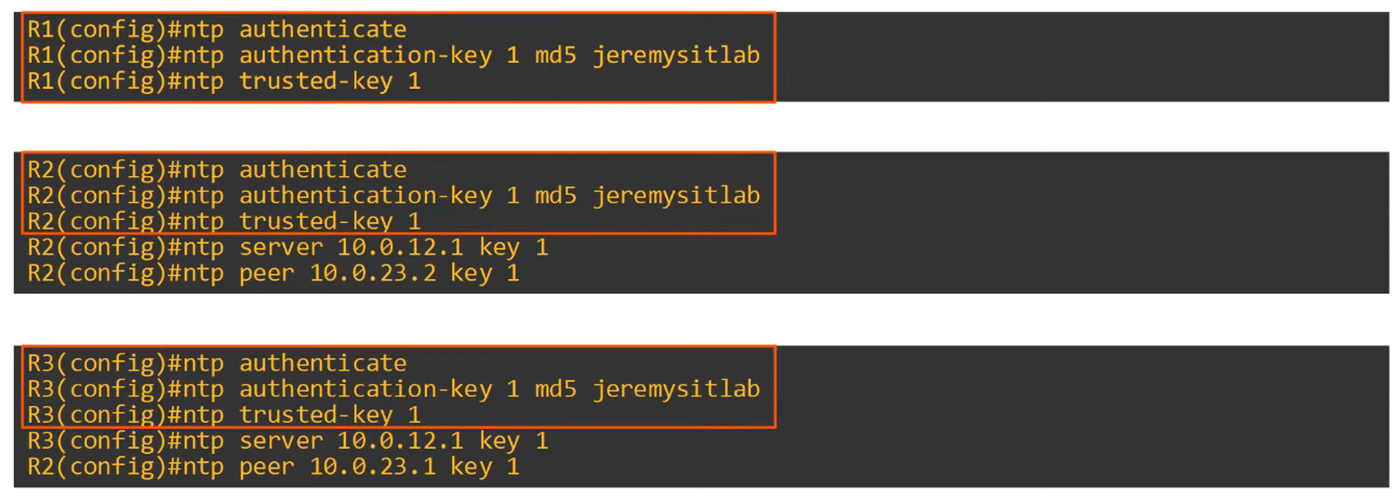
\includegraphics[keepaspectratio,alt={image}]{images/38-ntp/img-033.png}}
\end{figure}

\section{NTP Command Review}\label{ntp-command-review}

\begin{figure}
\centering
\pandocbounded{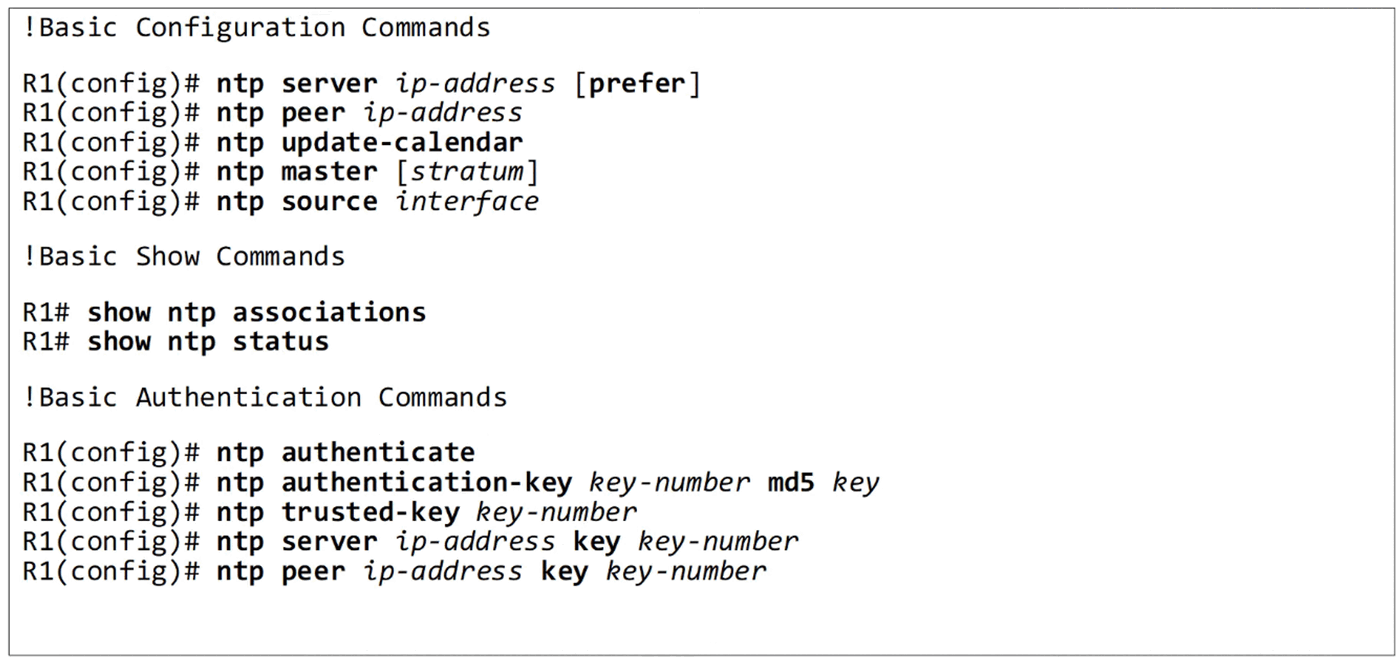
\includegraphics[keepaspectratio,alt={image}]{images/38-ntp/img-034.png}}
\end{figure}
